\scanpage{108}
\uline{Remarque.} Nous nous sommes bornés ici aux formules générales valables sans conditions de régularité (genre pseudo-cohérence, ou quasi-cohérence) qui \unsure{donnent|donneraient} de nombreuses autres formules. D'autre part, nous nous sommes bornés aux cas d'existence \inserted{``ordinaire'' i.e \unsure{générale}} des op. envisagées $\overset{\mathbb L}{\otimes}$, \inserted{$\mathbb Lf^*$}, $\mathbb R\mathcal Hom$, $\mathbb Rf_*$, sans examiner les variantes \unsure{provenant} d'hyp de Tor-dim ou Ext-dim. finie ....

\figure{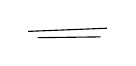
\begin{tikzpicture}\draw (0,0)--(1,.04);\draw (.12,-.08)--(.92,-.07);\end{tikzpicture}}

\textcircled{2} Formules \unsure{plus en particulières|un peu particulières}, faisant intervenir également $!$ en plus de $\overset{\mathbb L}{\otimes}$ : Künneth.

\deleted{\uline{Théorème} Soit $f:X\to Y$ un morphisme compactifiable. Alors pour}

Notons qu'en général, nous sommes obligés de travailler avec des faisceaux d'anneaux constants $\mathbb Z/n\mathbb Z=A$ qui n'est pas un corps ni de Tor-dimension \inserted{globale} finie, donc dès qu'on commence à faire des $\overset{\mathbb L}{\otimes}$, \deleted{\unsure{et}} en partant avec des faisceaux réduits au degré $0$, on va tomber dans $D^-$. Il faut
\mspage{107}
